\documentclass{report}

\usepackage{bindpage}
\usepackage{epsfig}
\usepackage{verbatim}

%
%  YAeHMOP Manual 
%   version 0.1 begun August 24, 1994  by greg Landrum
%   version 1.0 finished May 1, 1995 gL
%   version 1.1a started July 25, 1995 gL
%   version 1.2 finished Feb 26, 1996 gL
%   version 2.0 started Oct 18, 1996 gL
%
%   version 3.0 started August 1998, Wingfield Glassey
%   viewkel docs added back in March 2001, gL
\newcommand {\prog} {\mbox {\bf {\sf YAeHMOP\ }}}
\newcommand {\calcprog} {\mbox {\bf {\sf bind\ }}}
\newcommand {\viewprog} {\mbox {\bf {\sf viewkel\ }}}
\newcommand {\oldprog} {\mbox {\bf {\sf new3\ }}}
\newcommand {\cacao} {\mbox {\bf {\sf cacao\ }}}
\newcommand {\huek} {\mbox {H\"{u}ckel\ }}
\newcommand {\pvar}[1] {\mbox {\sl #1\ }}
\newcommand {\genprog}[1] {\mbox {\bf {\sf #1\ }}}
\newcommand {\resumespacing} {\baselineskip = 14pt}
\newcommand {\shrinkspacing} {\baselineskip = 12pt}

\begin{document}

\fontsize{12}{14}\selectfont

\title{ Yet Another Extended H\"{u}ckel Molecular Orbital Package \\
 (YAeHMOP) \\
 Version 3.0 User Manual}

\author{Greg Landrum and Wingfield Glassey}

\maketitle

\tableofcontents

\newpage

%%%%%%%%%%%%%%%%%%%%%%%%%%%%%%%%%%%%%%%%%%%%%%%%%%%%%%%%%%%%%%%%%%%%

\chapter{What is \prog\ and why should I use it?}

\prog\ is a group of programs for performing extended \huek\
calculations \cite{eht1,eht2} and analyzing and visualizing the results. 
The programs \calcprog\ and \viewprog\ form the core of the package.

\section{\calcprog}

\calcprog\ is the program which performs the actual extended
\huek\ calculations.  It can be used to perform calculations on both
isolated molecules and extended systems of 1, 2, or 3 dimensions. 

\calcprog\ is an almost complete rewrite of the program \oldprog\
and is written almost entirely in C (the routines for
evaluating overlap matrix elements and diagonalizing the
Hamiltonian matrix from \oldprog\ remain)
Because of the fact that all memory
used in the program is allocated dynamically, there are no
restrictions on the number of atoms, K points, or orbitals which can
be used (this isn't totally true:  there is a limit of 20 user defined
atom types).  The only limitation is the amount of memory that your
computer has and the length of time which you are willing to wait for
the run to finish.

Because of the fact that \calcprog\ is written to be easy to
maintain and understand, we have not spent a lot of
time trying to make it fast.  This isn't to say that it's slow, but it
certainly could be faster.

The input files to \calcprog\ are keyword based, so, with a few
exceptions, it doesn't really matter what order things are in.  In
addition, white space (spaces, tabs, etc.) in the input are ignored.

Here are just a few reasons to use \calcprog:
\begin{itemize}

\item Built in parameters for most elements.

\item Gaussian style Z--matrix, standard Cartesian, or
crystallographic coordinate input. 

\item Automatic generation of points along a reaction coordinate (for
Walsh diagrams).

\item Particular pieces of information can be monitored at each step
along a reaction coordinate (e.g. the reduced overlap population
between two atoms can be printed at each step along a Walsh diagram).

\item Automagic generation of K points along symmetry lines for band
structures.

\item Orientation independent determination of symmetry elements.

\item More symmetry elements are found (up through S$_8$).

\item DOS and COOP data are in ASCII format, so you can plot the data
with any plotting program... though you will {\em want} to use
\viewprog\ :-).

\end{itemize}

%%%%%%%%%%%%%%%%%%%%%%%%%%%%%%%%%%%%%%%%%%%%%%%%%%%%%%%%%%%%%%%%%%%%

\section{\viewprog}

\viewprog\ is an X--Windows based, interactive program for displaying
and printing the results obtained using \calcprog\ (though there's no
reason that it can't be made to display data from other programs).

Some of \viewprog's features are:

\begin{itemize}

\item Interactive 3-D manipulation of molecular structures.

\item Support for extended systems: ``grow'' crystals of any size.

\item Postscript output.

\item It doesn't use Motif.

\item Ability to place as many structures and graphs as desired on the same page. 

\item Numerous options for displaying molecules and MO surfaces.

\item Automatic generation of input files for \genprog{rayshade}, a
freeware raytracing program.  This can be used to get extra gratuitous
color 3D plots.

\item The official Roald Hoffmann seal of approval on the way the output looks.
 ({\bf NOTE:} this feature is still under development.)

\end{itemize}

Both \calcprog\ and \viewprog\ were written to be as easy to port to
other flavors of UNIX as possible.  This is one of the
reasons why \viewprog\ doesn't use any of the snazzy user interface
libraries which are available.




%%%%%%%%%%%%%%%%%%%%%%%%%%%%%%%%%%%%%%%%%%%%%%%%%%%%%%%%%%%%%%%%%%%%
\chapter{What's new in version 3.0?}

Quite a few new features have been added to \prog\ and one or two
'problems' have gone away :-) 

\noindent The \prog\ development team has also increased in size as of
this release ... so please
use the version 3.0 citations when publishing
results generated with \prog. Thanks ! \\[0.1in]


\noindent Additions to \calcprog\ include ...

\begin{itemize}

\item f-orbitals ... at last !!!

\item COOP's in a fragment molecular orbital (FMO) basis

\item Hamilton population analysis: a tool for total energy partitioning
built on the orbital, atom and fmo COOP options offered in \prog \cite{cohp1,cohp2,cohp3}

\end{itemize}

\noindent also the 'known bugs' section of the 'those damn bugs' chapter of the version 2.0 manual has vanished ... so there are absolutely {\bf NO} bugs left in \prog\ :-) \\[0.1in]



%%%%%%%%%%%%%%%%%%%%%%%%%%%%%%%%%%%%%%%%%%%%%%%%%%%%%%%%%%%%%%%%%%%%

\chapter{What's new in version 2.0?}

A bunch of stuff has been added to this version.  This is almost
certainly the last non-bug fix release of the programs until I
graduate.

\begin{itemize}

\item Numerous bug fixes.

\item Much improved MO plotting.  Including Jorgenson and
Salem (or CACAO) style plots that can be rotated in ``real-time'' to
find the optimal viewing angle.  Also included are contour plots
of MOs.

\item Fragment Crystal Orbital analysis, a new interpretive tool
for crystalline systems.

\item A new keyword allowing diagonalization of the hamiltonian
without including the overlap matrix.

\item \viewprog\ now provides distances, angles, and dihedral angles
between selected atoms in molecules.

\item There are several new options for display of molecules in
\viewprog.  Including tube bonds and pseudo-3D crosses.

%\item Support for independently defined ``Geometry Fragments'' in
%\calcprog.  These can be used to define complicated pieces of a molecule or
%crystal or to break a geometry definition into both cartesian and
%Z-matrix input.


\end{itemize}

%%%%%%%%%%%%%%%%%%%%%%%%%%%%%%%%%%%%%%%%%%%%%%%%%%%%%%%%%%%%%%%%%%%%

\chapter{What's new in version 1.2?}

\begin{itemize}

\item Support for using LAPACK routines to diagonalize the matrices. 

\item A version for Power Macs.

\item I have more faith in the MO drawings now.  The normalization
constants were right and now that I evaluate them in atomic units the
pictures look right too.  Thanks Grisha!

\item More juicy raisins in every bite!

\item Other things that escape me at the moment.

\end{itemize}





\chapter{Overview of how a calculation is done}

So you've come up with a cool problem (or it was assigned in class),
and you want to do an extended \huek\ calculation using \prog.  The
goal of this section is to get you familiar with the basic process for
moving from initial idea to final graphs and pictures.

The first step is to set up your input file. 
Basically, the input file contains a specification of the 
geometry of your molecule or extended system,
 the number of electrons in the system, any special information needed 
(the ranges of Walsh variables, any special parameters you may want to use,
 etc.) and any printing options that you want to set. \\[0.1in]



\noindent Here's a minimal input file example called {\tt foo.bind}


\shrinkspacing
\begin{verbatim}
; the name of the job
A silly example: a square of H atoms

; specification that this is a molecular problem
Molecular

;the geometry
geometry
4
1 H 0.0 0.0 0.0
2 H 1.0 0.0 0.0
3 H 1.0 1.0 0.0
4 H 0.0 1.0 0.0

; The number of electrons
Electrons
4

; printing options
PRINT
Overlap Population
Reduced overlap population
charge matrix
wavefunction
end_print
\end{verbatim}
\resumespacing


\noindent The contents of this file will be explained later. \\[0.1in]

\noindent To run the file execute the following command:

{\tt bind foo.bind}

This will create two output files: {\tt foo.bind.status} has some
status information; {\tt foo.bind.out} has all the results in it.

That's it!

If you had done a Walsh diagram or an average properties calculation
then there are some utility programs that need to be run to get the
data in shape to be displayed.  These will be discussed a later.

The data and results are now ready to be displayed using \viewprog\ or
your favorite plotting program.


\chapter{The input file}

Like many other programs, the input file for \calcprog\ is based on
keywords.  This allows the file to be broken into logical 
blocks and makes the format for constructing the file a little
less rigid.  Each keyword is described below.  Note that the input
routine (the parser) is
not case sensitive when dealing with keywords, i.e. Electrons,
electrons, and ELECTRONS will all work.

Any line in the input file which begins with a semicolon is ignored.
This allows comments to be put into the input file. It also makes it
easy to temporarily change the contents of a file, just put a
semicolon in front of anything you don't want the program to read.
Blank lines and spaces in the input are also ignored. \\[0.1in]

\noindent The first non-empty line should contain the title of the job.


\section{Keywords}
The remainder of the file contains the keywords which control the job.
These keywords are all described below.

The notation used is as follows:  

\begin{itemize}

\item Words in sans-serif style, such as {\sf foo,} are keywords.

\item Words in slanted type, such as \pvar{bar}, are
variable names used within the program.  They are used for convenience.

\end{itemize}


%%%%%%%%%
\subsection{{\sf Geometry} (required)}

The line following this keyword should have the number of atoms:
\pvar{num\_atoms}. 

If the line containing the keyword {\sf Geometry} also contains the
string {\sf Z Matrix} then the input is take to be in Gaussian style Z
matrix format.  If the line containing {\sf Geometry} also contains
the string {\sf Crystallographic} then the input is taken to be in
fractional coordinates and the {\sf Crystal Spec} keyword must be
specified.  Otherwise the input is assumed to be in Cartesian
coordinates.  If you are unfamiliar with Z matrix input, it is
described in a later chapter of this document.

The following \pvar{num\_atoms} lines should contain the atomic
coordinates and types in the following fashion:

\begin{itemize}

\item Z-matrix Input:  \pvar{number} \pvar{atom\_label} \pvar{ref1}
\pvar{r} \pvar{ref2}  \pvar{alpha} \pvar{ref3} \pvar{beta}

\item Cartesian Input: \pvar{number} \pvar{atom\_label} \pvar{X}
\pvar{Y} \pvar{Z}

\item Crystallographic Input: \pvar{number} \pvar{atom\_label} \pvar{X}
\pvar{Y} \pvar{Z}

\end{itemize}

\pvar{number} is the number of the atom.  There is no reason why the
atoms in the list have to be in increasing numeric order.

\pvar{atom\_label} is the label for the atom, it should be one or two
characters long.  If the atom label is a single asterix ({\tt *}),
then the atom is taken to be a custom type and a symbol and
parameters should be provided for it in the {\sf Parameters} section.
If the atom label is an ampersand ({\tt \&}), then the atom is taken
to be a dummy atom.

The other variables are the coordinates for the atom in whatever
system is being used.  If a reaction coordinate is being traced out
(see keyword {\sf Walsh} below), any coordinate which is an integer
multiple of 1000 is assumed to be variable.  For example: placing 2000
as the \pvar{X} coordinate of some atom would cause that coordinate to
take on the values of the second Walsh variable.


%%%%%%%%
%XXX  new XXX
%\subsection{{\sf Geom frag} (optional)}

%This keyword is used to specify a geometry fragment: a group of atoms
%that will be inserted as a single unit into the geometry of the unit
%cell.  

%%%%%%%%
\subsection{{\sf Lattice} (mandatory for extended systems)}

{\bf NOTE:} If this keyword appears in the file it {\em must} follow
the {\sf Geometry} keyword in the input file.

These are the lattice parameters.
The keyword should be followed by a line containing the dimensionality
of the crystal.  The next line contains the number of overlaps
considered along each lattice direction. The following lines should
contain the lattice vectors in the form:  \pvar{atom1} \pvar{atom2},
where \pvar{atom1} is the beginning of the vector (it is inside the
unit cell) and \pvar{atom2} is the end of the vector (it is outside
the unit cell).

{\bf NOTE:}  The ends of the lattice vectors must be the highest
numbered atoms in the geometry specification. For example, if there are
are 6 atoms defined for a 3 dimensional unit cell, then the ends of
the three lattice vectors must be numbers 4, 5, and 6.

Only a number of lattice vectors equal to the dimensionality of the
crystal need to be provided.  If you feel like putting in zeroes for
the other lattice vectors, go ahead... we can't stop you.



%%%%%%%%
\subsection{{\sf Crystal Spec} (required for use of crystallographic
coordinates)} 

This section has the stuff needed to define the crystal lattice so
that crystallographic coordinates can be used.

The first line following the {\sf Crystal Spec} keyword should contain
the lengths of each of the lattice vectors.  The next line should
contain the crystallographic angles $\alpha, \beta$ and $\gamma$.

Variables in the {\sf Crystal Spec} section can be used as variables
in Walsh diagrams in exactly the same way as variables in the {\sf
Geometry} section, i.e. by using integer multiples of 1000 as values.

For example, the following {\sf Geometry}, {\sf Lattice} and {\sf
Crystal Spec} 
sections define a body centered lattice of H atoms where the length of
the c lattice vector is the first Walsh Variable.

\clearpage

\shrinkspacing
\begin{verbatim}

Geometry Crystallographic
5
1 H 0 0 0
2 H 0.5 0.5 0.5
3 H 1 0 0
4 H 0 1 0
5 H 0 0 1

Lattice
3
5 5 5 
1 3
1 4
1 5

Crystal Spec
; a  b  c
  1  1  1000
; alpha  beta  gamma
   90     90     90

\end{verbatim}
\resumespacing


%%%%%%%%
\subsection{{\sf Electrons} (potentially required)}

The line following this keyword should have the number of valence
electrons in the molecule (or unit cell for an extended system).

%%%%%%%%
\subsection{{\sf Charge} (potentially required)}

The line following this keyword should have the charge on the molecule
(or unit cell for an extended system). \\[0.1in]

\noindent {\bf Either the {\sf Charge} or {\sf Electrons} keywords must appear in the
input file.}

%%%%%%%%
\subsection{{\sf Alternate Occups} }

This keyword is for looking at the effects of changing the number of
electrons in the unit cell upon the position of the Fermi level, the
average energy, and orbital occupations.  This is a far more efficient
way of probing these changes than rerunning the calculation with
alternate electron numbers.

On the line following the keyword, the number of alternate occupations
(\pvar{num\_occups}) should be given.  The next line contains the step
that is to be taken between occupations.

For example, the following input fragment would result in the program
doing a calculation with 5 electrons, then printing out the Fermi
level, average energy, net charges, and orbital occupations for
4.8,4.6,4.4,4.2, and 4.0 electrons per unit cell.

\shrinkspacing
\begin{verbatim}

Electrons
5

Alternate Occup
; num_occups
5
; the step
-.2
\end{verbatim}
\resumespacing



%%%%%%%%
\subsection{{\sf Parameters} (optional)}

{\bf NOTE:} If this keyword appears in the file it {\em must} follow
the {\sf Geometry} keyword in the input file.

There should be a line following this keyword for each type of custom
atom which is being defined.  Recall that a custom atom is defined by
replacing the first occurance of that atom's label in the Geometry
specification with an asterix: {\tt *}. If there are multiple custom
atom types, then define them in this section in the order in which
they occurred in the Geometry section. \\

\noindent The format of a parameter specification is:

{\small \pvar{Symbol} \pvar{Atomic\_Number}
\pvar{Num\_Valence\_Electrons} 
\pvar{n$_s$} \pvar{$\zeta_s$} \pvar{IP$_s$}
\pvar{n$_p$} \pvar{$\zeta_p$} \pvar{IP$_p$}
\pvar{n$_d$} \pvar{$\zeta1_d$} \pvar{IP$_d$} \pvar{c1}
\pvar{$\zeta2_d$} \pvar{c2}} \\

\noindent and if you're dealing with f-elements (which, like d orbitals, are described by a double zeta expansion) add:
{\small \pvar{n$_f$} \pvar{$\zeta1_f$} \pvar{IP$_f$} \pvar{c1}
\pvar{$\zeta2_f$} \pvar{c2}}
to the end of the parameter specification. \\

\noindent In this specification, the $\zeta$ values are the radial exponents of
the Slater type orbitals and the H$_{ii}$ values are the valence state
ionization potentials (diagonal elements of the hamiltonian) for each AO.
Here's an example of a section of input file where 3 different custom
atoms are defined:

\shrinkspacing
\begin{verbatim}

Geometry
8
1 *     .000000000     .000000000     .000000000
2 O    1.952000000    1.952000000     .000000000
3 *    1.952000000     .000000000    -.3
4 O    1.952000000     .000000000    1.4862
5 *    0.000000000    1.952000022    1.9422
6 O    3.904000044     .000000000     .000000000
7 O     .000000000    3.904000044     .000000000
8 O     .000000000    0.0                4.152

Parameters
O  8 6 2 2.275 -32.3 2 2.275 -14.8
Ti 22 4 4 1.075 -8.970 4 1.075 -5.400 3 4.55 -10.81 .4206 1.400 .7839
Pb 82 4 6 2.50  -16.70 6 2.06 -8.000

\end{verbatim}
\resumespacing
 
In this example, atom 1 is an O, atom 3 is a Ti, and atom 5 is a Pb.
Atoms 2,4,6,7, and 8 will use the same parameters as atom 1.  {\bf
Clarification:} The parameters specified here for O are the default
parameters. 


%%%%%%%%
\subsection{{\sf Molecular} (mandatory for molecular calculations)}

Indicates that a molecular calculation (not an extended one) is being
performed.  Otherwise it is assumed that the calculation is on an
extended system.

%%%%%%%%
%\subsection{{\sf Thin} (optional)}

%Do a THIN mode extended calculation.  This is not yet implemented, it
%will be added later to allow calculations to be run on machines with
%little available memory.

%%%%%%%%
%\subsection{{\sf Fat} (optional)}

%Do a FAT mode extended calculation.  This is the default for the
%program.

%%%%%%%%
\subsection{{\sf Just Geom} (optional)}

Do not actually do a calculation, just generate the molecular
geometry.  This is useful to check whether or not an input file is
okay before running a calculation.  It will also print the estimated
memory requirements of \calcprog\ for this run into the status file.


%%%%%%%%
\subsection{{\sf Walsh} (optional)}

Do a series of calculations along a reaction coordinate. 

The next line should contain the number of variables (reaction
coordinates): \pvar{num\_Walsh\_var}, and the number of steps to be taken
along each coordinate: \pvar{num\_steps}.  There should then be
\pvar{num\_Walsh\_var} lines consisting of a list of comma separated
\pvar{num\_steps} 
values.  

To generate the values of a variable automagically, place an
exclamation point ({\tt !}) at the beginning of the line for that
variable followed by the starting and ending values of the variable,
separated by a comma.
The program will generate \pvar{num\_steps} values between those
values.  

For example, the following sample section will generate a
reaction with coordinate with 5 steps and 2 variables.  The values of
the first variable will be automatically generated between 1.0 and
2.0, the values of the second variable are specified explicitly.

\shrinkspacing
\begin{verbatim}

Walsh
; the number of variables and number of steps
2 5
; use Auto-Walsh for the first variable:
! 1.0,2.0
100.0,100.1,100.2,100.3,100.4

\end{verbatim}
\resumespacing

Please note that, while there are two Walsh variables, they are varied
simultaneously.  There is not, at this point, a capability to vary the
Walsh variables independently in order to automatically generate a
multi-dimensional potential energy surface.

%%%%%%%%
\subsection{{\sf Symmetry} (optional)}

Find and report all the symmetry elements possessed by the molecule.
The 
characters of all wave functions with respect to these operations will
also be reported. 

{\bf Note:} As is explained in the section of this manual on symmetry
elements, {\calcprog} does not actually find {\em all} symmetry
elements.  It only finds those which are aligned with the Cartesian
axes. You can increase the number of symmetry elements which the
program finds by making sure that it align with the axes in a
reasonable manner.

%%%%%%%%
\subsection{{\sf Symm Tol} (optional)}

Allows the user to adjust the value of the tolerance used
for determining whether or not symmetry elements are present
in the molecule.  

The next line should contain the new value of \pvar{symm\_tol}.

If the position of an atom after a symmetry operation differs from
that of an atom before the symmetry operation is applied by less than 
\pvar{symm\_tol} \AA, then the two atoms are considered to be equivalent
under the symmetry operation.

%%%%%%%%
\subsection{{\sf Principle Axes} (optional)}

Determine the center of mass and principle axes of the molecule and
transform the atoms into the principle axis frame.  This can allow the
program to find more symmetry elements.  

{\bf Note:} Principle axes are only found if the {\tt meschach} library
was linked with \calcprog.  If you do not have {\tt meschach}, then
the program will just translate the molecule into the center of mass
frame before finding symmetry elements.

%%%%%%%%
\subsection{{\sf Zeta} (optional)}

Toggles self consistent variation of radial exponents.  This is under
development and if you don't know what it means, you probably
shouldn't be using it.

%%%%%%%%
\subsection{{\sf Nonweighted} (optional)}

Use the non-weighted H$_{ij}$ form \cite{wolfsberg}. 
By default the weighted H$_{ij}$
form is used in order to reduce problems arising from
counter--intuitive orbital mixing (gasp!) \cite{com1,com2}.

%%%%%%%%
\subsection{{\sf The Constant} (optional)}

Allows replacement of the value \pvar{K} used in evaluating the H$_{ij}$
elements.  The next line should contain the new value for \pvar{K}.
By default \pvar{K}=1.75.

%%%%%%%%
\subsection{{\sf Zero Overlap} (optional)}

Set some elements of the overlap matrix to zero.  The next line should
contain the number of different types of overlap being set to zero
(\pvar{num\_to\_zero}).  The next \pvar{num\_to\_zero} lines should
consist of:

\pvar{type} \pvar{contrib1} \pvar{contrib2} \pvar{which}

\pvar{type} should be either {\tt Atom} or {\tt Orbital} to indicate
which type of overlap is being zeroed.  If \pvar{which} is set to {\sf
Intercell}, then overlaps between \pvar{contrib1} and \pvar{contrib2} 
{\em between} cells will be zeroed.  If \pvar{which} is set to {\sf
Intracell} then the overlaps {\em inside} the cell will be zeroed.

{\bf NOTE:}  This option should be used with caution, as it can result
in a non-positive-definite overlap matrix and non-physical results.

%%%%%%%%
\subsection{{\sf Nearest Neighbor Contact} (optional)}

Determines the longest contact between atoms in nearest neighbor cells
that 
will be reported in the output file.  The next line should contain the
new value.  The default is 2.5 \AA. \\

\noindent {\bf NOTE:}  This keyword only makes sense for extended systems.

%%%%%%%%
\subsection{{\sf K Points} (mandatory for Average Properties
calculations on extended systems)}

A K point set for an average properties calculation.  If you want to
do a band structure, we recommend that you use the {\sf Band} keyword.

The keyword is followed by a line containing the number of K points:
\pvar{num\_KPOINTS}.   The next \pvar{num\_KPOINTS} lines should contain
the coordinates and weights of the K points themselves in the
following form:

\pvar{a} \pvar{b} \pvar{c} \pvar{weight} \\

\noindent Each K point should go on its own line.

%%%%%%%%
\subsection{{\sf Band} (optional)}

Generate a band structure.

The line following the keyword should contain the number of K points
to use along each symmetry line: \pvar{points\_per\_line}.

The next line should have the number of special points to be used:
\pvar{num\_special\_points}. 

The following \pvar{num\_special\_points} lines should have the names
and locations of the special points in the form:

\pvar{label} \pvar{x} \pvar{y} \pvar{z}

The program will generate symmetry lines connecting the special points
in the order in which they are defined.  \pvar{points\_per\_line} K
points will be generated automatically along each of these symmetry
lines.  The program will produce an additional output file containing
the information needed by \viewprog\ to plot the band structure.  If
your input file is called {\tt foo.bind}, then the band file will be
called {\tt foo.bind.band}.

For example, the following segment will generate a band diagram with
symmetry lines containing 40 K points running from $\Gamma$ to X to M and
then back to $\Gamma$:

\shrinkspacing
\begin{verbatim}

Band
; the number of points along each line
40
; the number of special points
4
Gamma 0.0 0.0 0.0
X     0.5 0.0 0.0
M     0.5 0.5 0.0
Gamma 0.0 0.0 0.0

\end{verbatim}
\resumespacing

%%%%%%%%
\subsection{{\sf FMO} (optional)}

Perform Fragment Molecular Orbital analysis.

The next line should contain the number of fragments
\pvar{num\_FMO\_frags}.  Note that \pvar{num\_FMO\_frags} should be
$\geq 1$.  There is no upper limit on the number of fragments.

The next line consists of a comma delimited list of the number of
electrons in each fragment.

The following \pvar{num\_FMO\_frags} lines consist of comma delimited
lists of the numbers of the atoms in each fragment.

In the specification of atoms for each fragment, you can use a hyphen
(dash) to indicate groups of sequentially numbered atoms.
For example, the following segment will generate 2 fragments, the
first fragment containing atoms 1, 2, 3, 4, 5 and 8 and the second fragment
containing atoms 6 and 7. \\


\shrinkspacing
\begin{verbatim}

FMO
; the number of fragments
2
; the number of electrons in each fragment
12,2
; the lists of atoms contained in each fragment
1-5,8
6-7

\end{verbatim}
\resumespacing

If a molecular calculation is being done, the data necessary to
construct an FMO interaction diagram will be written to a separate
output file.

%%%%%%%%
\subsection{{\sf FCO} (optional)}

Perform Fragment Crystal Orbital analysis.
The lines following this keyword are identical to those for the {\sf
FMO} keyword.


%%%%%%%%
\subsection{{\sf Average Properties} (optional)}

Do an average properties calculation for the system.  This consists
of:

\begin{itemize}

\item Generating a total DOS curve.

\item Finding E$_f$, the Fermi energy.

\item Determining the average overlap population and reduced overlap
population matrices within the unit cell (if the printing option for
these is set).

\item Finding average orbital occupations and net charges.

\item Reporting the average values of any COOPs specified (see
keyword {\sf COOP}).

\item Show average occupations of Fragment MO's (if FMO analysis is
being done).

\end{itemize}

\noindent {\bf NOTE:} if you are doing an average properties calculation on an
extended system, you
{\em must} provide a set of K points, see keyword {\sf K Points}.

Specifying an average properties calculation for a molecular problem
will allow the generation of MOOP (Molecular Orbital Overlap
Population) diagrams and the RCM (Reduced Charge Matrix) as for
extended syatems.

%%%%%%%%
\subsection{{\sf No Total DOS} (optional)}

Turns off printing of the total DOS into the output file.  This option
can be used to conserve disk space when the total DOS isn't going to
be looked at.  

{\bf Note:}  If this keyword is specified neither total DOS nor
projected DOS calculations will be done.


%%%%%%%%
\subsection{{\sf Dump Overlap} (optional)}

Toggles creation of a binary file containing the overlap matrix at
each K point.  This file can be used with the {\tt matrix\_view} utility to
generate pictures of overlap matrices.

%%%%%%%%
\subsection{{\sf Dump Hamil} (optional)}

Toggles creation of a binary file containing the hamiltonian matrix at
each K point.  This file can be used with the {\tt matrix\_view} utility to
generate pictures of hamiltonian matrices.

%%%%%%%%
\subsection{{\sf Dump Dist} (optional)}

Toggles creation of a binary file containing the distance matrix
for the system.  This .DMAT file can be used by the utiltity
{\tt cooperate} to generate specifications for COOPs automatically.


%%%%%%%%
\subsection{{\sf Projected DOS} (optional)}

This section contains the list of densities of states (DOS's) that
will be projected.  Each DOS can have multiple contributions which
will be added up.

The keyword is followed by a line containing the number of different
projections: \pvar{num\_proj\_DOS}. The next \pvar{num\_proj\_DOS} lines
should consist of:

\pvar{type} \pvar{contrib1} \pvar{weight1}, \pvar{contrib2}
\pvar{weight2},...

\pvar{type} should be either {\tt Atom}, {\tt Orbital}, or {\tt FMO} to indicate
whether the contribution from an entire atom, a single orbital, or a
fragment MO is being projected out.

There can be as many contributions to each projection as
you like, just put it all on one line and separate the
\pvar{contrib}--\pvar{weight} pairs by commas.
Entries for a single projection can be spread over multiple lines by placing a ``$\backslash$'' at the end of each line.
To {\bf average} contributions make the sum of the individual
contributions add up to 1.0.  To {\bf add} contributions, make each of
the contributions 1.0.  In general, it is a good idea to add projected
DOS curves rather than average them.

%%%%%%%%
\subsection{{\sf COOP} (optional)}

Do a Crystal Orbital Overlap (or Hamilton) Population analysis \cite{eht2,cohp3,mulliken,coop}. {\bf Note:} the {\sf COOP} option results in a Molecular Orbital Overlap (or Hamilton) Population analysis when the {\sf molecular} keyword is specified.

\noindent The line following the keyword has the total number of COOPs
specified (not just the number of different types): \pvar{tot\_num\_COOPs}.

\noindent The next \pvar{tot\_num\_COOPs} lines should contain the definitions
of the COOPs themselves in the form:

\pvar{type} \pvar{which} \pvar{contrib1} \pvar{contrib2} \pvar{a}
\pvar{b} \pvar{c} \\

\noindent \pvar{type} should be either {\tt Atom}, {\tt Orbital} or {\tt FMO} to indicate
whether the COOP between atoms, orbitals or fragment MO's is being projected. \\

\noindent Setting \pvar{type} to {\tt H-Atom}, {\tt H-Orbital} or {\tt H-FMO} will generate the corresponding Hamilton population between atoms, orbitals or fragment MO's respectively. \\

\noindent \pvar{which} is the number of the COOP.  Multiple COOPs with the same
value of \pvar{which} will be averaged. \\

The COOP reported is between \pvar{contrib1} in the unit cell and
\pvar{contrib2} in a cell defined by the vector (\pvar{a} \pvar{b}
\pvar{c}).  For example, the following sample section will average 
the COOP between atoms 1 and 2 in the unit cell with that between atom
2 in the unit cell and atom 1 in the adjacent cell in the \pvar{b}
direction:

\shrinkspacing
\begin{verbatim}

COOP
; the total number of lines here:
2
; definitions of the COOPS
;type  which  contrib1  contrib2     a b c
Atom    1       1          2         0 0 0
Atom    1       2          1         0 1 0

\end{verbatim}
\resumespacing

\noindent {\bf Note:}  If you are doing a COOP calculation on a high-symmetry
system where you are using K points within the irreducible wedge of
the first Brillouin zone, it is very important that you average all
symmetry equivalent bonds \cite{thesis}.
If you do not do so, your results may be inaccurate.

%%%%%%%%
\subsection{{\sf Printing} (optional)}

This keyword controls what information is printed into the output
file.  In most cases, this also controls what things the program
actually calculates.  For example, if the user doesn't request that
the reduced overlap population matrix be printed, then there's no
reason to calculate it.  We have tried to make the program
``smart'' about what it calculates, but, there
may be problems here.  Please let us know if you see strange behavior.

This keyword is different from all the others in that the program
expects it to be followed by another list of keywords.  In fact, any
keyword following {\sf Printing} is assumed to be controlling what
gets printed.  The way to tell \calcprog\ that you are done giving it
printing options is to either let it hit the end of the file (i.e. to
have {\sf Printing} as the last keyword in your input file, or to put
the keyword {\sf End\_Print} at the end of the printing options. \\

\noindent Each of the printing keywords is described below.

\begin{itemize}

\item {\sf Distance:}
Print the distance matrix.

\item {\sf Overlap Population:}
Print the Mulliken overlap population matrix.

\item {\sf Reduced Overlap Population:}
Print the Mulliken reduced overlap population matrix.

\item {\sf Charge Matrix:}
Print the charge matrix.

%\item {\sf Reduced Charge Matrix:}
%Print the reduced charge matrix. {\bf NOTE:} this is not yet
%implemented.

\item {\sf Wave Functions:}
Print the wavefunctions for the molecule.

\item {\sf Net Charges:}
Print the net charges on the atoms, as determined using Mulliken
population analysis.

\item {\sf Overlap:}
Print the overlap matrix.

\item {\sf Hamil:}
Print the hamiltonian matrix.

\item {\sf Electrostatic:}
Print the electrostatic contribution to the total energy.  {\bf NOTE:}
this is under development and is not to be considered reliable.

\item {\sf Levels:}
Toggles the printing of energy levels at each k point in an extended
calculation. 

\item {\sf Fermi:}
Print the Fermi energy (this is primarily useful in combination with
the Walsh option, described below). 


\item {\sf Orbital Energy:}
Allows the energy of a particular orbital to be printed.  (this is
primarily useful in combination with 
the Walsh option, described below). 

\item {\sf Orbital Coeff:}
Allows the coefficient of a particular atomic orbital in a given
molecular orbital to be printed.  (this is
primarily useful in combination with 
the Walsh option, described below). 

\item {\sf Orbital Mapping:}
Generates the scheme used to number the individual atomic orbitals in a calculation (especially useful when working out the contributions for COOP's)

\item {\sf Levels}
Print out the calculated energy levels at each k point in an extended
calculation. 
\end{itemize}

Each of these options control printing at every K point and/or step
along a reaction coordinate.  Turning on all the printing options can
lead to a {\bf huge} output file if you have a lot of K points or
steps in a Walsh diagram.

Placing the keyword {\sf Transpose} after a printing option for a
matrix will result in the transpose of the matrix being printed.  This
feature has been introduced to appease those who think that the default
way of printing is stupid.

To facilitate the construction of graphs of various quantities
(overlap populations, net charges, etc.) along a reaction coordinate,
there is a second option that can be used with printing options.  If
you place the keyword {\sf Walsh} on the same line as a printing
option, then you can select a particular quantity to monitor along the
Walsh diagram.  These values are put into a separate file.  If you are
using an input file named {\tt foo.bind} then the values of these
quantities would be put into {\tt foo.bind.walsh}.

To use this feature, place {\sf Walsh} after your
printing keyword, then on the next line put the following three pieces
of information:

\pvar{type} \pvar{contrib1} \pvar{contrib2}

Once again, \pvar{type} is one of {\tt Atom}, {\tt Orbital} or {\tt FMO} and
\pvar{contrib1} and \pvar{contrib2} refer to particular atoms,
orbitals or fragment MO's.

{\bf NOTE:} there are certain combinations of these Walsh printing
options which do not make sense.  For example, specifying that you
want to monitor the reduced overlap population between 2 orbitals is
nonsensical.  The program will notice this and complain, so just think
a bit before you start printing everything out.

For example, the following section would print out the entire overlap
population matrix and all the net charges at every step into the main
output file, and then
print the overlap population between orbitals 13 and 23 into the Walsh
output file:

\shrinkspacing
\begin{verbatim}
; start dealing with printing options
Print

Overlap Population
Net charges

; this is a Walsh printing value
Overlap Population   Walsh
Orbital 13 23

End_Print
\end{verbatim}
\resumespacing


%%%%%%%%
\subsection{{\sf MO Print} (optional)}

This keyword controls creation of a .MO file.  This can be read in by
\viewprog\ to produce iso-surface plots of molecular and crystal
orbitals.

The first line following the keyword contains the number of MO's to be
printed: \pvar{num\_MOs}.  The next \pvar{num\_MOs} lines contain the
numbers of the individual MO's that should be printed.

If you are doing an extended calculation, the MO's will be printed at
each k point.  If you are doing a Walsh diagram, the MO's will be
printed at each step along the reaction coordinate.  


%%%%%%%%
\subsection{{\sf Orbital Occupations} (optional)}
This section is used to change the occupations of molecular orbitals.
This is primarily useful for trying to model open shell systems or
molecules in excited states.  

The first line following the keyword should contain the number of
orbital occupations to change, \pvar{num\_occups}.  The next
\pvar{num\_occups} lines consist of an integer specifying the orbital
whose occupation should be changed and a real number specifying what
the new occupation should be.

For example, the following piece of an input file would place 1
electron in both orbitals 49 and 50:

\shrinkspacing
\begin{verbatim}

Orbital Occupations
; the number of occupations to change
2
; the orbitals and new occupations
49 1.0
50 1.0
\end{verbatim}
\resumespacing

%%%%%%%%
\subsection{{\sf Charge Iteration} (optional)}

\calcprog\ has the capability to perform charge iteration
(a self consistent adjustment of the H$_{ii}$s in order to lessen the
amount of charge flow).  
The charge iteration algorithm in \calcprog is somewhat experimental (... so beware!) and is discussed in the file {\bf charge.ps}.

For those of you who know no fear here's a summary of the CI keywords:

The keywords controlling the CI process are sandwiched between the {\sf charge iteration} and {\sf end charge} keywords.

The keywords within the CI block are: 

{\sf Param}
followed by a line giving the number of different atoms that parameters
will be specified for: \pvar{num\_CI\_parms}
each of the next \pvar{num\_CI\_parms} lines should contain the charge
iteration parameters in the form:
\pvar{Atomic\_symbol  $s_A s_B s_C p_A p_B p_C d_A d_B d_C$}

(i.e. the A, B, and C parameters for each of the orbitals.  These are
the same parameters used in the old programs for single configuration
CI and are NOT distributed with YAeHMOP).
{\bf Note:} charge iteration for f orbitals is not supported.

{\sf Vary}(follows Param)
followed by a single line containing the numbers of the atoms
whose parameters are to be varied. This is a comma delimited list, you
can use ``-'' to abbreviate series of atoms (i.e. 1-4 and 1,2,3,4 are
equivalent)

{\sf Tolerance}
followed by a single line specifying the tolerance used to terminate the iteration

{\sf lambda}
followed by a single line specifying the step size for the iteration process

{\sf max iter}
followed by a single line specifying the maximum number of iterations


%%%%%%%%
\subsection{{\sf Sparsify} (optional)}

This is used to set small elements of the hamiltonian and overlap
matrices to zero.  
The next line should contain the value which is considered to be zero.

{\bf NOTE:} This is primarily here for development purposes and 
we'd encourage you not to use this.

%%%%%%%%
\subsection{{\sf Just Average E} (optional)}

Tells \calcprog\ to only generate the average energy, total DOS, and
Fermi level of
the system.  This causes the program to require considerably less
memory when run on systems with a lot of orbitals.

If you are using a version of \calcprog\ that uses the
LAPACK libraries to diagonalize the matrices, then only 
eigenvalues will be generated.  This can result in a significant speed
increase.  (A factor of 10 decrease in execution time for
sufficiently large systems is possible !).

%%%%%%%%
\subsection{{\sf Just Matrices} (optional)}

Generate just the overlap and hamiltonian matrices, then exit.  This
is basically useless unless it is used in conjunction with either the
{\sf Dump Overlap} or {\sf Dump Hamil} keywords, or the {\sf
Hamiltonian} or {\sf Overlap} printing options.

%%%%%%%%
\subsection{{\sf Diagwo} (optional)}

Performs the matrix diagonalization without using the overlap matrix,
so that a calculation is similar to a simple H\"uckel calculation.




%%%%%%%%%%%%%%%%%%%%%%%%%%%%%%%%%%%%%%%%%%%%%%%%%%%%%%%%%%%%%%%%%%%%
\chapter{Symmetry analysis}

The symmetry analysis performed by \calcprog\ is relatively extensive
and flexible.  While the program doesn't find all
of the symmetry elements possessed by molecules, it does get a lot of
them. 

In order to make the symmetry analysis as flexible as possible, the
molecule can first be moved to the center of mass frame of reference. 
The 
moments of inertia are then found and the whole molecule is rotated
into the principle axis frame.  This allows molecules which are not
located exactly at the origin or aligned perfectly with the Cartesian
axes to be analyzed.  

The transformation to the principle axis frame is controlled by the
keyword {\sf Principle Axes}.  If this keyword is not specified, the
symmetry analysis will be done in the orientation specified in the
{\sf Geometry} section.

The program searches for the following
symmetry elements:

\begin{itemize}

\item {\bf an inversion center}

\item {\bf rotation axes} from C$_2$ through C$_8$ about the three
Cartesian axes.

\item {\bf improper rotation axes} from S$_3$ through S$_8$ about the
three Cartesian axes.

\item {\bf mirror planes} perpendicular to the Cartesian axes.

\end{itemize}

The elements found, their axes, and atoms which are equivalent under
each operation are printed to the output file.

The characters of the wavefunctions with respect to each operation are
determined by constructing the appropriate transformation matrix for
each operation and transforming the vector of atomic orbital
coefficients for each molecular orbital.  The result of this process
is the actual character of the wavefunction with respect to the
symmetry operation, not just a symmetric/anti-symmetric label.
It is important to realize that the results of this method of
displaying the results of symmetry analysis can give results which
are, at first, confusing for degenerate orbitals.  If you are looking
at the characters of a set of degerate orbitals and trying to compare
them to the characters given in a character table, it is very
important that you sum the characters of each of the members of the
degenerate set.


When a reaction coordinate is being followed, \calcprog\ first
generates all the geometries along the coordinate and determines the
symmetry elements which they possess.  The only symmetry elements
reported are those which are conserved along the entire distortion.
This means that you don't have to worry about moving from high to low
symmetry geometries or {\it vice versa}.  {\bf Note:} It is possible
that loss of symmetry elements will lead to problems in constructing a
Walsh diagram.  In these cases {\bf {\sf fit\_walsh}} will warn you.
If the diagram as constructed is incorrect, you can either change your
reaction coordinate to not include geometries with problematic
degeneracies or edit the {\tt .WALSH} file by hand to fix it.  This is
explained in more detail below in the section on fitting programs.

%%%%%%%%%%%%%%%%%%%%%%%%%%%%%%%%%%%%%%%%%%%%%%%%%%%


\chapter{\prog\ on the Macintosh}

As of version 1.2 of \prog, there is a Macintosh port of everything.
At the moment, the Mac version only runs on Power Macs.
A port to the 68K based Macs is not suported.

%There hasn't been much testing of \prog\ on Power Macs
%configured differently than what we have in the group, but it's a fairly
%safe bet that \viewprog\ will not work on displays that have
%less than 256 colors available.  There's also a distinct possibility
%that it won't work on displays with more than 256 colors.  To be safe,
%go to the Monitors control panel and switch to 256 color mode before
%running \viewprog.

The Mac port was done using the CodeWarrior compiler from Metrowerks.
Source code and project files for the Metrowerks IDE are available
upon request.
Codewarrior is fantastic ! Metroworks prices it reasonably, includes a ton of
useful examples and libraries, and has an
excellent upgrade policy.  In addition, the MW technical support is
{\bf excellent}.

The Fortran bits of the program were converted using f2c on our
workstations, and then compiled on the Mac using a port of the f2c
libraries.  All input and output that would normally go to the
console on a workstation is handled by the SIOUX library included with
CodeWarrior.  The basic structure of the graphics stuff used in
\viewprog\ was done using the EasyApp application shell distributed
with CW.

\section{A couple of disclaimers}
The Mac version of \prog\ is not the most beautiful thing that the
world has ever seen.  Some of the operations are handled in an ugly,
non-Mac way.  This is a direct consequence of the program's
Unix heritage.  Hopefully, in some future version these 
difficulties will be eliminated.

The Mac version of the programs are not nearly as stable as the UNIX
version, principally because the MacOS isn't a
protected mode operating system.

\section{Using \calcprog\ on a Macintosh}

When \calcprog\ starts up it will open a standard file choice dialog,
you should choose the input file in that dialog box.  If the program
has problems opening the parameter file (usually called {\tt
eht\_parms.dat}), it'll pop up another dialog box.  You should use that
dialog box to find and select the parameter file.  You can avoid this
by having a copy of the parameter file in the same folder as the input file.
To work around this make an alias for {\tt eht\_parms.dat}, copy it to 
the input folder, and then rename it {\tt eht\_parms.dat}.

%\section{Using \viewprog\ on a Macintosh}

%While the Mac version of \viewprog\ is very similar to the X version,
%there are a few differences:
%\begin{itemize}
%\item Instead of having button windows open up, new menus are added to the
%menu bar.   

%\item When opening files, you will not be prompted for the file
%name, but will be given a standard Mac file choice dialog.

%\item Filling of projected DOSs is not done on screen.
%If curve filling is turned on, the printed output will
%be filled properly.

%\item Line styles are indicated with color on screen.  This is because
%Quickdraw doesn't seem to support dashed line styles.  The Postscript
%files generated still use dashed line styles like on the Unix version.

%\item Breaking lines and tube bonds are not always drawn properly on screen.
%This is due to another problem with Quickdraw, which does not define
%line thicknesses relative to the center of the line.  Again, the
%Postscript output is fine.

%\item Standard mac printing isn't up and running yet, but you can still
% create a postscript file and print that just as you would print any
% postscript file from the mac.  
%This will probably be fixed in a future version.

%\item Because the Mac mouse only has a single button, some of the
%selection features work differently.  You must be in {\sf Select} mode
%to change active objects.

%\end{itemize}


\section{The fitting programs}

The fitting programs will open a file choice dialog on start up.  You
should pick the {\em input} file used to run the calculation.

\section{General Mac hints}

If you get errors about the programs not having enough memory or not
being able to allocate matrices, increase the size of the memory
allocation for the troublesome program.  If you don't know how to do
this:  select the application you want to change, select ``Get
Info'' from the File menu (or hit CMD-I), then increase the
``Preferred Size'' entry. 
%%%%%%%%%%%%%%%%%%
%%%%%%%%%%%%%%%%%%




\chapter{Sample Extended System Input File}

This is an input file for doing a band structure and average
properties calculation on a square 2 dimensional mesh of hydrogen
atoms.

\vspace{0.25in}

\shrinkspacing
\begin{verbatim}
; the title
2-D mesh of hydrogen

; the geometry
Geometry
; number of atoms
3
; the positions
1 H 0.0 0.0 0.0
2 & 1.0 0.0 0.0
3 & 0.0 1.0 0.0

; lattice parameters
Lattice
; dimension of lattice
2
; number of overlaps along each lattice vector
4 4
; the lattice vectors (begin atom -> end atom)
1 2
1 3

; number of electrons per unit cell
Electrons
1

; band structure details
Band
; K points per symmetry line
40
; number of special points
4
; special points
Gamma 0.0 0.0 0.0
X     0.5 0.0 0.0
M     0.5 0.5 0.0
Gamma 0.0 0.0 0.0

; do average properties calculation
Average Properties

; do a COOP
COOP
; number of COOP's
2
; COOP specifications
; type  which    contrib1 contrib2   cell
orbital  1          1         1      1 0 0
orbital  1          1         1      0 1 0

; this averages H-H COOP's between cells (0,0,0)->(1,0,0) and (0,0,0)->(0,1,0)

; the K points
K points
; number of K points
10
; the K points and respective weights
0.0625 0.0625 0.0000 1
0.1875 0.0625 0.0000 2
0.1875 0.1875 0.0000 1
0.3125 0.0625 0.0000 2
0.3125 0.1875 0.0000 2
0.3125 0.3125 0.0000 1
0.4375 0.0625 0.0000 2
0.4375 0.1875 0.0000 2
0.4375 0.3125 0.0000 2
0.4375 0.4375 0.0000 1

; end of file
\end{verbatim}
\resumespacing



%%%%%%%%%%%%%%%%%%
%%%%%%%%%%%%%%%%%%
\chapter{The Fitting Programs}

In order to generate nice looking DOS and COOP curves, it is necessary
to either use hundreds of k points in the calculation or to smooth the
data which is 
generated by \calcprog.  For obvious reasons, it is far more common
to adopt the latter approach.

Smoothing of DOS and COOP curves is done by putting a gaussian on each
data point, then summing up the contributions from each of the
gaussians between the data points.  This process gives rise to the
type of curves we are used to seeing.

The parts of \prog\ which perform this smoothing operation are called
{\tt fit\_dos} and {\tt fit\_coop}.  These both take the name of the
input file which was given to \calcprog\ as an argument.

Here is a sample session:

\shrinkspacing

\begin{verbatim}

% bind H_mesh.bind
% fit_dos H_mesh.bind
Enter E min: -30.0
Enter E max: 30.0
Enter broadening: 10.0
Enter Energy Step: 0.5

\end{verbatim}

\resumespacing

The broadening parameter given to the fitting programs is the exponent
of the normalized Gaussian smoothing function.  A larger broadening
parameter gives rise to sharper lines in the DOS/COOP curves.

After this smoothing process, which produces either a {\tt .DOS} or
{\tt .COOP} file, the data is ready for viewing with \viewprog.

In order to view a Walsh diagram, the program {\tt fit\_walsh} must be
run.  {\tt fit\_walsh} is run the same way as {\tt fit\_dos} or {\tt
fit\_coop}: you give it the name of the input file which was given to
\calcprog.  If you lose symmetry elements along the distortion
coordinate and degeneracies are broken, it is possible that {\tt
fit\_walsh} will get confused and generate a silly looking Walsh
diagram.  {\tt fit\_walsh} will warn you if this happens.  If the
output looks wrong in \viewprog\, you can either manually edit the {\tt 
.WALSH} file created by {\tt fit\_walsh} or rerun the calculation with
more points along the distortion and use the program {\tt dumb\_walsh},
which ignores symmetry operations.  If you take the {\tt dumb\_walsh}
route, we recommend you use at least 30--40 points along the
distortion.  Hopefully a future version of the program will have a
smarter version of {\tt fit\_walsh} so that these contortions are no
longer necessary.



%%%%%%%%%%%%%%%%%%
%%%%%%%%%%%%%%%%%%
\chapter{Other Utility Programs}

There are a number of other utilities distributed with \prog.  These
are described below.

\section{sub\_dos and add\_dos}

These are used to manipulate .DOS files.  {\tt sub\_dos} is used to
subtract two DOS curves from each other.  This is the basic operation
needed for the Crystal Orbital Displacement (COD) analysis developed
by Eliseo Ruiz and Santiago Alvarez \cite{cod}. COD is a very sensitive tool for tracking complicated interactions in the solid state.  Running {\tt sub\_dos} without any arguments will give you the correct ordering of arguments.

{\tt add\_dos} is like {\tt sub\_dos} except that it adds two DOS
curves together.

{\bf Note:} It is very important that the DOS curves used for {\tt
sub\_dos} are fit (using {\tt fit\_dos}) within the same energy window
and with the same broadening and energy step.  The programs will warn
you about this.

\section{cooperate}

{\tt cooperate} reads in the .DMAT file generated when \calcprog\ is
given the keyword {\sf Dump Distance Matrix} and generates a COOP
specification that can be pasted into an input file for \calcprog.
The output from {\tt cooperate} needs very little modification before
incorporation into an input file.  The necessary modifications are
fairly obvious.  Once again, running the program without any arguments
will give you a complete list of possible arguments.




\chapter{Contents of Files}

The various programs in \prog{} produce different output files, the
names of the files may be confusing.

For a run on a file named {\tt example}, here are the names of
the files produced and the contents of those files:

\begin{itemize}

\item {\tt example.status}: status information about the job

\item {\tt example.out}: the main output file. Contains energies,
occupations, average properties, etc.

\item {\tt example.walsh}: the values of variables which were printed
out along each step of a reaction coordinate.

\item {\tt example.band}: the information needed by \viewprog{} for
constructing a band diagram.

\item {\tt example.DOS}: (generated by {\tt fit\_dos}) the information needed by \viewprog{} to
generate DOS curves.

\item {\tt example.COOP}: (generated by {\tt fit\_coop}) the
information needed by \viewprog{} to generate COOP curves.

\item {\tt example.WALSH}: (generated by {\tt fit\_walsh}) the
information needed by \viewprog{} to generate Walsh diagrams.

\item {\tt example.FMO}: contains the information needed by
\viewprog{} to generate FMO diagrams. 

\item {\tt example.MO}: contains the information needed by
\viewprog{} to generate MO pictures.

\item {\tt example.DMAT}: generated when the {\sf dump distance
matrix} keyword is used, contains the information needed by
{\tt cooperate} to automatically generate COOP specifications for
crystals. 


\end{itemize}


\chapter{Those Damn Bugs!}

One thing to be aware of is that \prog\ is under development, so there
are some features built into it which may or may not be permanent.
We've tried to indicate wherever possible when things are not finished
or are in the testing stages.


\section{What is a bug?}

There are two possible reasons for a calculation to screw up: a bug in
the program or a user error.  Please make sure that your input file is
correct before you send in a bug report.

Any of the following things could indicate a
bug:

\begin{enumerate}

\item \calcprog\ gives you answers that don't make any sense at all

\item \calcprog\ does something funny like not printing out something
you told it to print out.

\item \calcprog\ wanders off into space and never comes back (i.e. it
runs forever).

\item \calcprog\ crashes without giving you some idea of what
happened.

\item \calcprog\ seg faults and dies. (You see the message: {\tt
Segmentation Fault: core dumped})

\end{enumerate}

We have yet to see \calcprog\ do anything like \#3 above.  If you do
think that the run is taking too long, check the status file and make
sure that it is still doing something.

\calcprog\ should {\bf never} do either \#4 or \#5 above.  If either
of these happen you have definitely found a bug.  {\bf Please report it}.
The major cause of segmentation faults seems to be problems in the
input files given to \calcprog. Error checking routines are in place to
catch many of these problems, but we probably missed a
few.  So please let us know if you find input file formats that give
rise to segmentation faults without generating a warning.

\viewprog\ is a slightly different story.  The code for \viewprog\
isn't nearly as clean or carefully written as that in \calcprog.  The
result is that \viewprog\ occasionally will dump core and/or die
unexpectedly. We're aware of some of these problems and are working on
them.  If you can make \viewprog\ dump core reproducibly, please let
us know.  Similarly, if the output from \viewprog\ just looks wrong,
tell us and we'll see what we can do.

\section{What to do if you find a bug}

In order for us to be able to fix bugs, we have to be able to reproduce
the circumstances that gave rise to them.  In order to do this, we need
a copy of the input file that caused the problem.  Please include the
following in any bug report that you send:

\begin{enumerate}

\item A description of what went wrong, or why you think the answers
you got are wrong.

\item Copies of the input file (essential), and the status and output
files (optional, but extremely useful).

\item Information about what kind of computer you are using (machine
type and operating system version if possible).

\item Some way to get in touch with you.

\end{enumerate}

Please send bug reports to the following email address:

{\tt yaehmop@xtended.chem.cornell.edu}



%%%%%%%%%%%%%%%%
%%%%%%%%%%%%%%%%
%%%%%%%%%%%%%%%%
\chapter{ Some (hopefully) helpful hints}

\section{Choosing how many overlaps to use}

The overlaps specified determine how many unit cells the program
uses when building the overlap matrix in K space.
The important thing when answering this question is to remember that
the goal is to include all unit cells surrounding the 'home' cell 
that have a non-zero contribution to the overlap
matrix. The general criterion here is that you should
go out far enough that the length of the lattice vector times the
number of overlaps is between 10 and 20 \AA.  Some systems don't
require this many overlaps, and some require more.  It's safe to go
with too many overlaps, though this causes \calcprog\ to use more
memory and go slower.  If you don't have enough overlaps, the
diagonalization procedure will fail.  This will be reported in the
status file after the program finishes running.


\section{Choosing the number of k points to use}

This is a tricky question.  The right answer is that you should always
do a k point convergence test for every calculation (i.e. you should
try using a variety of different sampling densities and stop when you
get convergence).   However, this isn't always practical or possible.
The general guideline we use is that the number of crystal orbitals
(number of orbitals in the unit cell times the number of k points)
should be equal to 1000.  This criterion is highly questionable when
doing slab models of interfaces or surfaces, so be careful with these
systems.

\section{Choosing the number of points in band structures}

Generally using 40 k points per symmetry line works fine.  If your
bands are flat, you can use less than this.  If you are really worried
about seeing weakly avoided crossings and you can't tell if you are
seeing one, use more points.


\section{Calculations on big systems}

When doing calculations on large systems (where the meaning of large
depends on how much memory your computer has), it's very good idea to
do the average properties and band structure calculations separately.
This is because average properties calculations use a lot more memory,
and band structure calculations use a lot more k points.  If you are
nearing the limit of the memory available on your machine because of
the demands of the average properties calculation, the band structure
calculation will take much much longer than it has too.  You are
better off if you do the two runs separately.  It's also a good idea
to do the band structure once, then comment out the band part of the
input file.  That way if you add projected DOS's or COOPs later, you
won't accidentally redo the band structure, which won't have changed. 

%\section{Using \viewprog}

%When moving or scaling graphs (property, band, walsh, whatever) in
%\viewprog, it's a good idea to turn off the curves.  Everything will
%update a hell of a lot faster if you do.  Once you have everything in
%place, turn the curves back on. 

%The 3D perspective code in \viewprog\ is stupid and primitive.  It
%works okay, but the interface is clunky and it is lacking some
%features that should be there.  The biggest of these is the lack of
%near plane clipping.  What this means to you, the user, is that
%objects behind the camera which is showing you the image will show up
%on screen, they'll just be inverted.  To work around this problem,
%either move the molecule farther away from you, or adjust the Z
%scaling. 



\chapter{Using \viewprog}

\viewprog\ is written to display results on either X Windows displays
or Tektronix terminals.  The program will automatically detect whether
or not X Windows are available and will use them if they are.
Printing is handled by generating Postscript 
files which can then be directly printed or included in documents.
The actual graphics calls used to draw the data are all included in a
separate file, so it should be reasonably easy to port the program to
other graphics systems.

Since the use of the X and Tek versions of \viewprog\ is different,
they will be dealt with separately.

{\bf Note:}  I haven't put much work into the command line (Tektronix)
version of \viewprog\ recently, so it doesn't have a lot of the
features mentioned below and some of the features it purportedly does
have may not work.

\section{Using \viewprog\ in X}

When you start \viewprog\ under X, it will open 2 windows.  The first,
and larger, window (the graphics window) is used to display output.
The second window (the main button window) has buttons which are used
to control the program. 

The individual button windows and the functions of the buttons found
therein are described below.  Each button is only described once, so
though many different windows have a {\bf X Legend} button, it is only
described once. 

You can cause the program to redraw at any time (except when an
isosurface is being evaluated) by middle clicking in any of the
windows.

\subsection{Special keys in \viewprog}

There are a number of keys that can be used in \viewprog, some of
these duplicate features found in button windows, some are unique.

\begin{itemize}
\item {\bf q}: will cause \viewprog\ to quit.
\item {\bf r}: switches into rotate mode.
\item {\bf t}: switches into translate mode.
\item {\bf c}: switches into center mode.
\item {\bf s}: switches into scale mode.
\item {\bf the spacebar}: switches into choose mode.
\item {\bf h}: in choose mode hides the selected atoms
\item {\bf +}: in choose mode shows previously hidden atoms
\item {\bf z}: rotates the selected molecule so that you are looking
along the Z axis.
\item {\bf y}: rotates the selected molecule so that you are looking
along the Y axis.
\item {\bf x}: rotates the selected molecule so that you are looking
along the X axis.
\item {\bf 1}: \viewprog\ will prompt you for a file name to use, then
write an input file for {\tt rayshade}.
\item {\bf d}: writes the cartesian coordinates of the molecule to
standard output.
\end{itemize}


\subsection{General use of buttons}

In order to avoid having to use a user interface library that may not
exist on some machines, I wrote all the button code myself.  This
means that the buttons aren't necessarily the most beautiful things
you've ever seen, and sometimes they behave in ways which are just
plain wrong (for example, text can overflow out of the button).  The
most important thing from my perspective is that these buttons do
work, and the code to deal with them is simple and small.

To activate a button, left click on it.  If it is a toggle button,
then the toggle will be changed.  If the button is for changing the
value of some variable, you will be prompted to enter a new value for
that variable (no, I didn't write dialog box code).  

Buttons which are for toggling the display of lines will show a sample
of the line style to the right of the button.  You can change this
line style by right clicking in the toggle button.

\subsection{The main button window}

The buttons in the main button window are described below:

\begin{itemize}

%%%%%%%%%%%%%%%%%%
\item {\bf the Mode button}:  This is the top button in the window.
It displays what mode the program is using to manipulate the graphics
displayed in the graphics window.  Left clicking in this window
changes the active mode. This mode determines what action
the control keys have.  The control keys are i,j,k,l,p,and ;.  The
first four of these form an inverted arrow on a standard keyboard.  

The possible modes are:

\begin{itemize}
\item None:  the control keys do nothing.

\item Rotate:  the control keys rotate the active object.
i and k rotate about the y axis, j and l rotate about x, and p and ;
rotate about z.  Holding down shift while hitting any of these keys
results in a larger rotation step.  
In versions of \viewprog\ greater than or equal to 2.0, you can also
rotate molecules in rotate mode by left clicking and dragging in the
graphics window.  This is easier to do than it is to explain, so try
it out.
{\bf Note:}  Rotations only apply to displayed molecules and MO's, not
to graphs because that would be silly.


\item Translate:  the control keys translate the active object.
i and k move along the y axis, j and l move along x, and p and ;
move along z.  Holding down shift while hitting any of these keys
results in a larger step.  

\item Center:  the control keys translate the center of the active
object. 
i and k move along the y axis, j and l move along x, and p and ;
move along z.  Holding down shift while hitting any of these keys
results in a larger step. 
This is different from the {\sf Translate} mode for molecules and MO
surfaces in that the molecule and the point that the camera used to
construct the perspective view looks at are move simultaneously.  This
allows the molecule to be moved about the screen without the view
changing. 
In versions of \viewprog\ greater than or equal to 2.0, you can also
change the center of your molecule by left clicking in the graphics
window.  When you do this, the center of the molecule will be moved to
where you clicked.  If you then drag, the molecule will move.
{\bf Note:}  For anything other than molecules and MO surfaces {\sf
Translate} and {\sf Center} are equivalent.

\item Scale: the control keys change the size of the active object. 
j shrinks along x, l grows along x, k shrinks along y, i grows along
y, ; shrinks along z, and p grows along z.  Once again, holding down
shift while hitting a key increases the size of the step.

\item Choose: Left clicking on atoms selects them.  Right clicking
then either displays the distance between those atoms (two selected),
the angle between them (three selected), or the relevant dihedral
angle (four selected).  A label is placed at the location
of the right click and lines are drawn to the controlling atoms.  If
you right click with just a single atom selected, the coordinates and
identity of that atom will be printed in the window from which you ran
\viewprog.  This is a convenient way to find the coordinates of a
particular atom if you forget (or if you have centered the molecule
using the ``center'' button in the molecule option window).
The labels displayed in Choose mode remain on screen until the {\sf
Clear Labels} button is 
hit.  

\end{itemize}

%%%%%%%%%%%%%%%%%%
\item {\bf Read Molecule}:  Reads in the atomic positions of a
molecule.  You will be prompted for the name of the {\bf output} file
containing the geometry.  Enter the name of the file in the window
from which you started up \viewprog.  The molecule will be read in and
displayed and a molecule button window will be opened.

%%%%%%%%%%%%%%%%%%
\item {\bf Read MO}: Reads in the specification of an MO.  You will be
prompted for the name of the {\bf input} file used to perform the
calculation. Enter the name of the file in the window from which you
started up \viewprog.  The program will read in the geometry of the
molecule itself from the {\tt .out} file and the MO specification from
the {\tt .MO} file.  You will be prompted for which MO you which to
use if there are multiple MO's in the {\tt .MO} file.  {\bf Note:}  To
use this option you must have specified MO printing when \calcprog\
was run.   

%%%%%%%%%%%%%%%%%%
\item {\bf Read Contours}:  Reads in a contour plot.  You will be
prompted for the name of the file containing the contour data.
This option is primarily intended for dealing with FCO plots.

%%%%%%%%%%%%%%%%%%
\item {\bf Read FMO}:  Reads in FMO data and constructs an interaction
diagram.  You will be prompted for the name of a {\tt .FMO} file.
\viewprog\ will read in the FMO data, construct an interaction
diagram, and open an FMO options window.

%%%%%%%%%%%%%%%%%%
\item {\bf Read Props}:  Reads in average properties (DOS, COOP or
COD) data and displays it.  You will be prompted for the name of a
data file (either {\tt .DOS}, {\tt .COOP}, or {\tt .SUB}).  The
program will read in the data and open a property options window.

%%%%%%%%%%%%%%%%%%
\item {\bf Read Walsh}:  Reads in data for a Walsh diagram.  You will
be prompted for the name of a {\tt .WALSH} file.  \viewprog\ will read
in the data and open a walsh option window.

%%%%%%%%%%%%%%%%%%
\item {\bf Read Bands}:  Reads in the data to display a band
structure.  You will be prompted for the name of a {\tt .bands} file.
\viewprog\ will display and band structure and open a bands option
window.


%%%%%%%%%%%%%%%%%%
\item {\bf Read Graph}:  Reads in raw data for a graph.  You will be
prompted for the name of the file containing the graph data.  This
allows construction of very primitive graphs.  This option just exists
because it was easy to do.  \viewprog\ is not intended to be a general
purpose graphing program.

%%%%%%%%%%%%%%%%%
\item {\bf Fill Proj.s}:  Toggles filling of projected DOS curves.  On
screen these will be shown shaded, in the printed output they will be
lined.  {\bf Note:} in the Macintosh version of \viewprog, this
keyword has no effect on the way things are displayed on screen, it
does still affect the Postscript output.

%%%%%%%%%%%%%%%%%%
\item {\bf Purge!}: Deletes all currently displayed objects and closes
all of their button windows.

%%%%%%%%%%%%%%%%%%
\item {\bf Printing Options}:  Opens a window which allows you to
change some of the default behavior for the Postscript printing.


%%%%%%%%%%%%%%%%%%
\item {\bf Print}:  Prompts for the name of a file, then redraws the
screen, writing its contents to the file as Postscript.  This file can
then be printed however you normally print {\tt .ps} files.

%%%%%%%%%%%%%%%%%%
\item {\bf Clear Labels}:  Removes labels from the display.  They
will not be refreshed, so once you clear them, they are gone.

\end{itemize}


%%%%%%%%%%%%%%%%%%
%%%%%%%%%%%%%%%%%%
\subsection{The PS options button window}

This window allows you to control some of the default behavior of the
Postscript printing from \viewprog.  

\begin{itemize}
\item {\bf Location}:  This button controls where the graph is located
on the output page.  There are three possible values: Top, Middle and
Bottom.  The default is Bottom.

\item {\bf Font}: Allows specification of the standard text font.  The
default is Times--Roman.  {\bf Note:}  This option can be overridden
using the enhanced Postscript commands (described in an Appendix).

\item {\bf Font Size}: Allows specification of the standard text font
size (in points).  The default is 12.

\item {\bf Scale}: Allows scaling of the whole output.  This does {\em
not} affect the size of the text font, to change that use the {\bf Font
Size} button.

\end{itemize}

{\bf Note:} None of the changes
made in this window will be visible on screen.


%%%%%%%%%%%%%%%%%%
%%%%%%%%%%%%%%%%%%
\subsection{The molecule button window}

This is the window which is popped up when a molecule is opened.  It
is used to control the viewing options for the molecule being
displayed.  

\begin{itemize}
\item {\bf Hydrogens?}: Toggles drawing of hydrogens.

\item {\bf Dummies?}: Toggles drawing of dummy atoms.

\item {\bf Center}:  When this is pressed, the molecule is moved so
that it is centered at the center of mass ({\bf Note:} since
\viewprog\ doesn't actually know what the masses of your atoms are,
the center of mass is actually calculated assuming all the atoms have
the same mass.  The resulting positioning is usually still right.).


\item {\bf Hide Atoms} Allows you to make it so that some atoms in the
molecule aren't displayed.  You will be prompted for a list of atoms
to hide.  Enter a comma delimited list. You can use the dash (hyphen)
just as it was used in the FMO specification.  For example, the
following list will hide atoms 1-23 and 99:
{\tt 1-23, 99}

\item {\bf Show Atoms} Allows you to ``unhide'' atoms you may have hidden
before. 

\item {\bf Axes?}: Toggles display of a set of axes on screen.

\item {\bf Outlines?}: Toggles the drawing of dark circles around
the atoms being displayed.

\item {\bf Shading?}: Toggles shading of the atoms being displayed.

\item {\bf Crosses?}: Toggles display of pseudo-3D crosses on the
atoms.  If this is turned on and shading is turned off, the interiors
of the atoms are drawn as solid white with the cross superimposed.

\item {\bf Connectors?}: Toggles drawing of lines connecting atoms
which are a distance within \pvar{bond\_tol} (see below) of the sum of
their covalent radii apart.

\item {\bf Fancy Lines?}: When this is on lines between atoms are
drawn as if they are intersecting the sphere of the atoms.  When off,
the lines are drawn all the way to the center of the atoms.  Turning
``Fancy Lines'' off is useful when drawing a structure without the
atoms being displayed.

\item {\bf Breaking Lines?}: When this is turned on, lines ``cut'' those
behind them that they intersect.

\item {\bf Tube Lines?}:  Toggles display of bonds as tubes instead of
lines.  Tubes are drawn as a white center with a black edges and 
cut lines behind them just like breaking lines.  {\bf Note}: if both
``Tube Bonds'' and ``Breaking Lines'' are turned on, only the Breaking
Lines will be drawn.


\item {\bf Numbers?}: Toggles display of the numbers of atoms.

\item {\bf Symbols?}: Toggles display of atomic symbols.

\item {\bf Line Width}: Used to control the thickness of the lines
drawn between atoms.

\item {\bf Bond Tol}: Used to enter a new value of \pvar{bond\_tol}.
When this is changed the lines between atoms are recalculated.

\item {\bf Rad Scale}: Used to control the scaling of the circles
drawn for atoms.

\item {\bf Grow Xtal!}:  This button only appears for molecules that
have lattice parameters in the output file (i.e. extended systems).
Clicking this allows you to show more than one unit cell.

\end{itemize}

%%%%%%%%%%%%%%%%%%
%%%%%%%%%%%%%%%%%%
\subsection{The MO button window}

{\bf Note:} This section is substantially changed since \viewprog\
version 1.2.

When an MO isosurface is opened, two button windows are opened.  One
of these windows is a Molecule window as described above.  The other
window is used to control the drawing of MO isosurfaces on
screen.  These options are described below.

There are two ways to draw isosurfaces in \viewprog\ version 2.  The
first method draws the isosurface just as it was done in version 1.2:
a solid isosurface made up of filled triangles is drawn.  These
isosurfaces do not look particularly good when drawn in viewkel, but
generate very nice illustrations when {\sf rayshade} is used to
raytrace the object. The second method draws Jorgenson and Salem style
contour plots of the surface, with hidden line removal. These plots
are similar to those generated by {\sf CACAO} and {\sf PSI88}.  I will
refer to these as ``solid'' surfaces and ``contour'' surfaces
respectively.  Finally, this button window is also used to generate a
two dimensional contour plot of an MO, I'll refer to these as ``contour plots''.

While some buttons apply to both types of figures, the majority
control only solid {\em or} contour surfaces.

To explain what the solid surface buttons do, it is necessary to
understand how the calculation of solid isosurfaces is done.  The algorithm
used to generate the polygonal isosurface is taken from a section by
Jules Bloomenthal (at Xerox PARC) in the book {\em Graphics Gems IV}.
The algorithm as published is suitable for polygonalization of
continuous surfaces.  Unfortunately, isosurfaces of molecular and
crystal orbitals are rarely continuous.  They are, instead, made up of
a number of discrete parts (usually lobes centered on particular
atoms).  In order to work around this problem, Bloomethal's algorithm
has been modified to look for individual pieces of the surface around
each atom in the molecule.  The algorithm starts at the corners of a
cube of side length \pvar{search\_radius} centered on each atom.  The
default value of \pvar{search\_radius} seems to work most of the time,
if you see that lobes are obviously missing, try changing the value of
\pvar{search\_radius}.   The algorithm evaluates the MO values on a
grid of spacing \pvar{voxel\_size}.  Increasing \pvar{voxel\_size}
results in quicker evaluation and drawing of the surface (less
triangles are found, so the surface can be drawn more rapidly), but
the resolution suffers.  Decreasing \pvar{voxel\_size} gives a
smoother surface, but it takes much longer to calculate and to draw.
My best advice here is to start with the default value (0.2\AA) and
then play around with it to see what size suits your purpose.


{\bf Some Cautions about solid isosurfaces:} 

\begin{itemize}

\item I haven't had a
chance to do shading (simulated lights) of the isosurfaces.  I
think that this will improve the appearance of the final images.  

\item A heuristic needs to be developed to warn the user when lobes of
the MO might have been missed.  I have some ideas here, but I'm still
working on them.

\end{itemize}

When the surface is first read in, the user is prompted for values
used in constructing the radial lookup table.   This is a table of
values for the radial part of the wavefunctions.  Use of this lookup
table results in a tremendous gain in speed.  The default values
should be fine for almost any calculations.

One important note about {\em both} solid and contour isosurfaces: 
\viewprog\ does not deal with the imaginary part of 
wavefunctions yet.  I will put this in later, until then, limit
yourself to pure real wavefunctions.  You'll always be okay with
molecular wavefunctions, but general k points for extended systems
will be problematic.

Well, with my salvo of disclaimers fired, here are the explanations of
the buttons in the MO options window.

\begin{itemize}

\item {\bf Surface?}: Toggles display of the solid isosurface once it has
been calculated.

\item {\bf Molecule?}: Toggles display of the molecule.

\item {\bf Isosurface}: This is the isosurface value that is displayed
on screen.  This is applies to both solid and contour isosurfaces.

\item {\bf Voxel Size}: The spacing of the grid used to calculate the
solid surface.

\item {\bf Search Rad}: The size of the cube around each atom used to
provide starting points for the solid surface search.

\item {\bf Slop}:  Used to determine how far past the end of the
molecule's bounding box the solid isosurface grid extends.

\item {\bf Exclude Atoms}:  Used to remove atoms from the calculation
of the isosurface.  For example, if you are doing a 7 layer metal slab
and are only interested in the surface states (a topic near and dear
to my heart), you can exclude the atoms which are in the middle of the
slab.  This will result in a cleaner looking, more quickly evaluated
isosurface.  You will be prompted to enter a list of atoms, the syntax
here is the same as for the Hide Atoms button described in the
Molecule options section.

\item {\bf Include Atoms}:  This is used if you make a mistake when
you exclude atoms. It turns the atoms you switched off back on.

\item {\bf Surf Evolve}: Starts the calculation of a solid isosurface.

\item {\bf Change MO}:  Allows you to change which MO you are looking
at without having to reload the whole molecule.

\item {\bf Tri\_Shading?}: Toggles filling of the triangles which make
up the displayed solid isosurface.

\item {\bf Tri\_Outlines?}: Toggles the drawing of outlines around the
triangles which make up the solid isosurface.

\item {\bf Contours?}: Toggles display of the calculated contours that
make up either a contour plot of an MO or a contour isosurface.

\item {\bf Contour Mode}:  This mode button determines the method
which is used to generate contour levels in contour plots.  There are
three possibilities: {\sf Auto} \pvar{num\_contours} contour levels
are automatically selected between the maximum and minimum values in
the data set; {\sf Incremental}, you will be prompted for a starting
value and a step between contours when the contour plot is evaluated;
{\sf Discrete}, you will be prompted to enter the \pvar{num\_contours}
contour values when you evaluate the contour plot.  

\item {\bf Contour it}: Evaluates a contour plot.  You will be
prompted for:
\begin{itemize}
\item  the orientation of the plane used to evaluate the contours
(i.e. perpendicular to X, Y or Z)
\item  the height and width of the plane in which the MO will be
evaluated.
\item the number of steps to take along each side of the evaluation
plane.
\item the number of contours you want to use
\item an offset, this shifts the evaluation plane off the origin,
useful if you want to contour an MO where most of the density isn't at
X,Y, or Z = 0.
\item Whether or not you want to do a ``stack'' of contour plots.
  If you say yes here, you will be prompted for the number of planes
you want in the stack, the location of the start of the stack, and the
distance between planes in the stack.  What this does is generate a
series of plots which are parallel to each other and located at
different heights.  This is a quick and dirty way to get a feeling for
the shape of an MO.  {\bf Note:}  if the contour mode is {\sf Auto},
\viewprog\ will generate the contour levels automatically in the first
plane of the stack, but then will use those contour values in all
other planes.
\end{itemize}

\viewprog\ will then go off and evaluate the values of the MO in the
plane, contour that data, show you the values of the contours it
found, and finally display those contours (if the {\sf Contours?}
toggle described above is switched on).  MO contour plots are real
three dimensional objects just like the molecule they are associated
with, and will rotate, translate, and scale in three dimensions along
with the molecule.  This feature seems gratuitous, but it's kind of
fun to play with and it was a lot easier to implement than having the
contour be a fixed 2D object.  It can even be useful:  if you rotate
the molecule so that you are looking at the edge of the contour plot,
you can see exactly where it cuts through your molecule.

\item {\bf Contour Surf}: Evaluates an MO contour plot.

\item {\bf Invert Phase}:  This toggle allows you to invert the phase
of the MO displayed on screen.  This can be helpful when you want to
visually compare two similar MO's that have opposite phases: just
invert the phase of one of them.

\item {\bf Hidden}:  Toggles the use of the hidden line removal
algorithm for contour plots and MO surfaces.  When \pvar{Hidden} is
on, you should no longer be able to ``see through'' the MO isosurface.
However, this can make it take a lot longer to draw plots, so you may
want to have \pvar{Hidden} turned off when you are rotating your
molecule.  The hidden line removal does not work particularly well for
normal contour plots, but \viewprog\ will still allow you to use it if
you wish. {\bf Note}: there are still some boundary conditions that
get screwed up sometimes in the hidden line removal.  If a plot looks
bad: rotate the molecule a small amount, that should clear things up.
{\bf Very, Very Important Note}:  The hidden line removal algorithm is
not guaranteed to work at all if you have some contours displayed
which are not closed (this can arise if the plane in which you
evaluated the MO was too small).   Sometimes it works, sometimes it
does stuff that is very, very wrong.  

\item {\bf Grow Xtal}:  This grows the crystal and propagates the MO
coefficients with the correct phase factors for the given k point.  If 
you want to display the MO of an extended system in more than one unit
cell, you {\bf must} use this button to grow the crystal.  Using the
{\bf Grow Xtal} button in the Molecule button window will not
correctly propagate the MO coefficients.

\end{itemize}

{\bf Note:}  If are looking at an extended system, and you want to see
the crystal orbital in more than the home unit cell, you must
evaluate the isosurface after growing the crystal.


%%%%%%%%%%%%%%%%%%
%%%%%%%%%%%%%%%%%%
\subsection{FMO button window}

This window contains buttons for controlling the display of an FMO
interaction diagram.

\begin{itemize}
\item {\bf Electrons}:  Controls the drawing mode for the electrons in
the interaction diagram.  Each mode is described below:

\begin{itemize}
\item None: Do not draw electrons.

\item HOMO: Draw electrons only in the highest occupied level of each
fragment and the molecule.

\item All: Draw electrons in all occupied levels on screen.
\end{itemize}

\item {\bf Levels}: Toggles display of the levels in the FMO diagram.

\item {\bf Left Fragment}: Controls which fragment is displayed on the
left side of the interaction diagram.  Set this to zero or -1 to not
show a fragment on the left side.

\item {\bf Right Fragment}: Controls which fragment is displayed on the
right side of the interaction diagram.  Set this to zero or -1 to not
show a fragment on the right side.

\item {\bf Y min}: This is the minimum energy displayed.

\item {\bf Y max}: This is the maximum energy displayed.

\item {\bf Level Width}: The width (horizontal length) of the levels
drawn.

\item {\bf Thickness}: The thickness of the lines used to draw the
levels.

\item {\bf Electron len}: The length of the lines used to represent
electrons.

\item {\bf Y tics}: Toggles the display of tic marks on the y axis.

\item {\bf Frame}: Toggles the display of a frame around the
interaction diagram.

\item {\bf Show Title}: Toggles display of the title of the graph (if
one has been entered).

\item {\bf Title}: Allows you to enter a new title to be displayed
across the top of the graph.

\item {\bf Main Label}: Allows you to enter a new label for the
central set of levels (those of the full molecule).

\item {\bf Frag {\sf n} Label}: There will be one of these buttons for
each fragment used in the calculation.  These are used to enter labels
to be displayed under each fragment displayed.

\end{itemize}

%%%%%%%%%%%%%%%%%%
%%%%%%%%%%%%%%%%%%
\subsection{Walsh button window}

This window is used to control the display of Walsh diagrams.  The
coordinate used to label the x axis is specified when {\sf fit\_walsh}
is run.

\begin{itemize}

\item {\bf MO's}: Toggles display of the MO levels.

\item {\bf Total E}: Toggles display of the total energy.

\item {\bf X tics}: Toggles display of X tics.

\item {\bf MO tics}: Toggles display of Y axis tic marks (for the
energies of the MO's displayed) on the left side of the diagram.

\item {\bf Tot E tics}: Toggles display of Y axis tic marks (for the
total energy curve) on the right side of the diagram.

\item {\bf X Legend}: Allows you to enter a legend to be displayed
under the X axis.

\item {\bf Y Legend}: Allows you to enter a legend to be displayed
beside the Y axis.
\end{itemize}

%%%%%%%%%%%%%%%%%%
%%%%%%%%%%%%%%%%%%
\subsection{Band button window}

Controls the display of band structure data on screen.

\begin{itemize}
\item {\bf Bands}: toggles display of the bands.

\item {\bf Show Fermi}: toggles display of the Fermi energy on the
band graph.

\item {\bf Fermi E}: allows you to enter a value for the Fermi energy.
The location of the Fermi energy is not stored in the band file, so
you must enter this yourself to get an accurate value.
\end{itemize}

%%%%%%%%%%%%%%%%%%
%%%%%%%%%%%%%%%%%%
\subsection{Properties button window}

This is used to control display of average properties data (DOS, COOP,
or COD data).  

\begin{itemize}
\item {\bf Curve n}: where n is an integer.  This is a toggle to
control display of each curve in the file.  The numbering of the
curves varies from type to type:  
\begin{itemize}
\item DOS data:  Curve 1 is the total DOS.  Projections are
labeled starting from Curve 2.  The projections are in the order in
which they were specified in the input file.

\item COOP data: The curves are numbered in the same way as the COOPs
were numbered in the input file.

\item COD data: There is only one curve per COD file, this is curve 1.
\end{itemize}

\item {\bf Integration n}: where n is an integer.  These toggle
display of
the integration of the corresponding curve.

\item {\bf Integ Scale}: toggles use of the integration data to label
the X axis.  This is particularly useful for integrated DOS data.
There are problems with using this option for COOP and COD data.
These will be fixed in the next version of the program.

\item {\bf Fermi E}: allows you to change the value of the Fermi energy.
For DOS and COOP data the value of the Fermi energy is stored in
the output file, so \viewprog\ will know the proper value.  

\end{itemize}

%%%%%%%%%%%%%%%%%%
%%%%%%%%%%%%%%%%%%
\subsection{Graph button window}

This controls displays of graph data.  There are no new buttons for
control of graph data.

%%%%%%%%%%%%%%%%%%
%%%%%%%%%%%%%%%%%%
\section{Using \viewprog\ from a Tek terminal}

When you are sitting at a Tek terminal (Tek 4014 compatible),
\viewprog\ will use a command line driven interface and will use the
graphics capabilities of the terminal to display graphs. 

You can get help in the Tek version of the program by typing ``help''
or ``?'' at the prompt.  This will list all the commands along with a
brief description.  Since this is available, I will not describe all
the features here.

Though it can be convenient, the Tek interface does have some
limitations: 

\begin{itemize}
\item You can not look at either molecules or MO's.

\item Not all features of each type of graph are modifiable.

\item Once a new graph has been opened, previously opened (and
displayed) graphs cannot be modified.

\item Due to limitations of the technology, the graph you see onscreen
is not nearly as similar to what comes out of the printer as in
the X windows version of \viewprog.

\end{itemize}

{\bf Note:}  It has been a long time since I have worked on the
Tektronix version of \viewprog, so it's not guaranteed to work at all.

%%%%%%%%%%%%%%%%%%
%%%%%%%%%%%%%%%%%%


%%%%%%%%%%%%%%%%
%%%%%%%%%%%%%%%%
%%%%%%%%%%%%%%%%
\chapter{Using the enhanced Postscript features in \viewprog}

It is now possible to include superscripts, subscripts, different
fonts, and all kinds of other wacky stuff in output from \viewprog.
This is accomplished using an adaptation of the enhpost terminal type
from gnuplot.  If you are familiar with this, then you don't have to
read this section, everything is exactly the same here {\em except}
that you can't do rotated text.

To get a superscript, use the \^{} symbol.  \^{} only holds for one
character unless a group of characters is enclosed in squiggly
brackets (\{ and \}), so the line:
\begin{verbatim} 	X^10 \end{verbatim}
comes out looking like: 
\begin{quotation}
X$^10$,
\end{quotation}
while the line 
\begin{verbatim} 	X^{10} \end{verbatim} 
gives:
\begin{quotation}
X$^{10}$. 
\end{quotation}
To get a subscript, use the \_ symbol.  \_ behaves in the same manner
as \^\ . 

To change font, put a backslashed version of the name of the font
inside squiggly brackets with the text to be changed.  For example
\begin{verbatim} look at {/Symbol G} now \end{verbatim}  
gives: 
\begin{quotation}
look at $\Gamma$ now. 
\end{quotation}

There are some other features of the enhpost drivers, but these are
the most important.


%%%%%%%%%%%%%%%%%%
%%%%%%%%%%%%%%%%%%
\chapter{A word (or two) from Greg ... some acknowledgements}

The members of the Hoffmann group were invaluable in the development
and testing of these programs.  They provided moral support, bug
reports, featur suggestions, and esthetic criticisms that were
invaluable.  The group 
members most involved were: Hugh Genin,  Norman Goldberg, Kimberly
Lawler, Qiang Liu,  Erika Merschrod, Udo Radius, Grigoriy Vajenine
(who pointed out  
that I should be evaluating the radial parts of wavefunctions in
atomic units), and Kazunari
Yoshizawa.  In addition, the students and auditors of Chemistry 798 in
the fall of 1994 and the spring of 1995. acted as unwitting
beta-testers and uncovered a few   
problems I never would have found.  Roald Hoffmann (my advisor) was
very supportive of my efforts and never chastised me for how much
time I was devoting to this project.  Of course, he {\bf did} accuse
the program of being vaporware, but this should nip that criticism in
the bud.  Thanks Roald!   

Edgar M\"{u}ller has provided a number of helpful suggestions as well
as some Fortran code which served as the template for the
code to deal with crystallographic coordinates.  Edgar also came up
with a consistent parameter set for the entire periodic table.  This 
parameter set is distributed with this release of the program as {\tt
muller\_parms.dat}.

Paul K\"{o}gerler has also provided suggestions for features which are
now integrated and has even agreed to add some features himself.
Expect to see these in a future release.

The function used to diagonalize the inertia tensor as part of the
symmetry analysis is taken from the {\sf meschach} library.  This is a
freely available package of functions written in C for working with
matrices. {\sf meschach} was written by David Stewart and Zbigniew Leyk
at the Australian National University.  If you want to use this
function in your own code, please obtain a copy of the entire library.
I want to go ahead and 
take the chance to thank David Stewart for making this library freely
available.  At this point I can't help but interject a piece of 
propaganda: free software is top quality stuff, find out about it and
use it! 

The basis of the code to calculate solid isosurfaces was taken from
the article ``An Implicit Surface Polygonalizer'' by Jules Bloomenthal
in {\em Graphics Gems IV}, Academic Press, 1994.  If you do graphics,
taking a look at these books is a really good idea.  

The algorithm used to do hidden line removal in the Jorgenson and
Salem style MO plots is a slight modification of that used in
Jorgenson's {\sf PSI88} program.  Because {\sf PSI88} is written in
Fortran, none 
of the code from the program was used, I just used {\sf PSI88} to
figure out the algorithm.

The enhanced postscript code is adapted from the file enhpost.trm for
{\sf gnuplot} version 3.5.  The original code was written by David Denholm
and Matt Heffron, both of whom have given me permission to distribute
this adaptation. 

The code used to contour data (both for FCO and MO plots) is adapted
from that used in {\sf gnuplot} version 3.5 (I love borrowing code from
{\sf gnuplot}!).  The original code was written by Gershom Elber and this
modification is distributed with his permission.



\chapter{Using the LAPACK diagonalizer}

\calcprog\ can now use a function from the LAPACK library ({\tt
zhegv}) to diagonalize the hamiltonian.  This diagonalizer is
significantly faster than the default routine {\tt cboris}.  In
addition, {\tt zhegv} can be used to generate just the eigenvalues of
a matrix.  This speeds up band structure calculations and properties
calculations with the {\sf Just Average E} keyword enormously.  

If you have a binary distribution of the program, it will use {\tt
zhegv} to diagonalize (this is, unfortunately {\bf not} true of the
Mac version of the program, which still uses {\tt cboris}).  If you
have a source distribution, you can turn on the LAPACK diagonalizer by
including {\tt -DUSE\_LAPACK} in the {\tt CFLAGS} line of the
makefile.  Most of the functions necessary to use
LAPACK with \prog\ are distributed in the file {\tt zhegv.f}.
This is the good news.  
The bad news is that {\tt zhegv.f} will not work unless you
have an implementation of the Basic Linear Algebra Subroutines (BLAS)
library installed on your machine (this is why the Mac version doesn't
currently support LAPACK).  Most modern distributions of UNIX include
a specially tuned version of the BLAS library (it's usually {\tt
/usr/lib/libblas.a}), so you should be able to use LAPACK.  In
addition, many UNIX implementations will include (as an optional
product) a tuned version of LAPACK.  The name of this library is very
system dependant, so you'll have to determine if it exists (if you
have an SGI, it's {\tt /usr/lib/libcomplib.sgimath.so}).  If you do
have a vendor-supplied version of LAPACK, it's advisable to
use it instead of the {\tt zhegv.f} distributed with \prog, the
vendor product tends to be faster.

If you are willing to compile BLAS for your system, or if you want the
full LAPACK distribution, you can get them from the netlib server
({\tt http://netlib.att.com}).  Netlib is a {\bf great} source for
numerical routines.

%%%%%%%%%%%%%%%%
%%%%%%%%%%%%%%%%
%%%%%%%%%%%%%%%%
\chapter{Distributing and Modifying \prog}

You can distribute \prog\ to anybody you like.  It's intended to be
given away.  However, you cannot charge others for the distribution.
We are firm believers in free software, and would like \prog\ to
remain freeware.

The programs which make up \prog\ are available in source form.  If
there is a feature lacking which you feel really should be there, feel
free to add it.  If you think that others might like to use this
feature, let us know and we'll see about integrating it into the main
distribution.  This is much easier if you clearly indicate in the
source code where you have made changes and, if possible, send a
context sensitive diff of the modified source files.  If you find and
fix bugs, please do the same thing.



%%%%%%%%%%%%%%%%
%%%%%%%%%%%%%%%%
%%%%%%%%%%%%%%%%
\chapter{Updates}

\prog is still under development.  The next version will contain bug fixes
and other great stuff.  If you send us 
email (yaehmop@xtended.chem.cornell.edu) and let us know that you have
the program, we can send you mail and let you know when the next
version is done.  If you don't let us know that you have the program,
you'll just have to keep checking our anonymous ftp site ({\sf
ftp://overlap.chem.cornell.edu/dist/yaehmop}) or the \prog\ home page
on the World Wide Web ({\sf
http://overlap.chem.cornell.edu:8080/yaehmop.html}). 


\chapter{Citing \prog}

If you publish calculations and/or figures that you produce using either
\calcprog or \viewprog, we'd appreciate it if you'd cite the program 
in your references section.  
At this point, there are no print publications describing
\prog, so there's no obvious citation to give. \\[0.2in]

\noindent Please use the following citation for \calcprog:

\noindent G.A.Landrum and W.V.Glassey, \calcprog (ver 3.0).
\calcprog is distributed as part of the \prog extended H\"{u}ckel molecular orbital package and is freely available on the WWW at;

{\it http://sourceforge.net/projects/yaehmop/} \\[0.2in]

\noindent and the following citation for \viewprog:

\noindent G.A.Landrum, \viewprog (ver 3.0).
\viewprog is distributed as part of the \prog extended H\"{u}ckel molecular orbital package and is freely available on the WWW at;

{\it http://sourceforge.net/projects/yaehmop/} 



\chapter{Specifying your geometry with a Z-Matrix}

A Z-Matrix is a convenient way to specify the geometry of a molecule or
crystal in terms of bond lengths, bond angles, and dihedral angles.
There are several styles of Z-matrix used in various programs,
\calcprog\ uses a format similar to that used in Gaussian.
This is intended to be a brief introduction to how a Z-matrix works.

If you already know how to use a Z-matrix, here's all you need to know
about the implementation in \calcprog:
\begin{itemize}
\item The first atom is put at the origin.
\item The second atom is put along the Z axis.
\item The third atom is in the XZ plane.
\item Dihedrals are evaluated using the right hand rule.
\end{itemize}

The easiest way to explain a Z-matrix is to show one and then explain
it, so that's what we'll do.  Before we start, however, we need to
briefly define a dihedral angle.  A dihedral is specified by 4
atoms, we'll call them A, B, C, and D.  The dihedral A--B--C--D is the
angle between the plane defined by A--B--C and the plane defined by
B--C--D.
Here's an alternative explanation: the dihedral A--B--C--D is the angle
between the lines C--D and B--A if you are looking down the line C--B.
There's one more piece of information we need to fully understand the
dihedral: there is a handedness associate with them.  If you think
about it, looking down the line C--B there are two different angles
between lines C--D and B--A: $\theta$ and 360-$\theta$.  The dihedrals
in \calcprog\ are defined using the right hand rule:  Take your right
hand and point the thumb down the line C--B, now align your fingers
with the line C--D, curling your fingers shows the direction in which
the dihedral angle is measured.
%
This is all about a million times easier to understand using a
picture, here's a picture demonstrating both views of dihedrals and
their handedness. 
%
\begin{center}
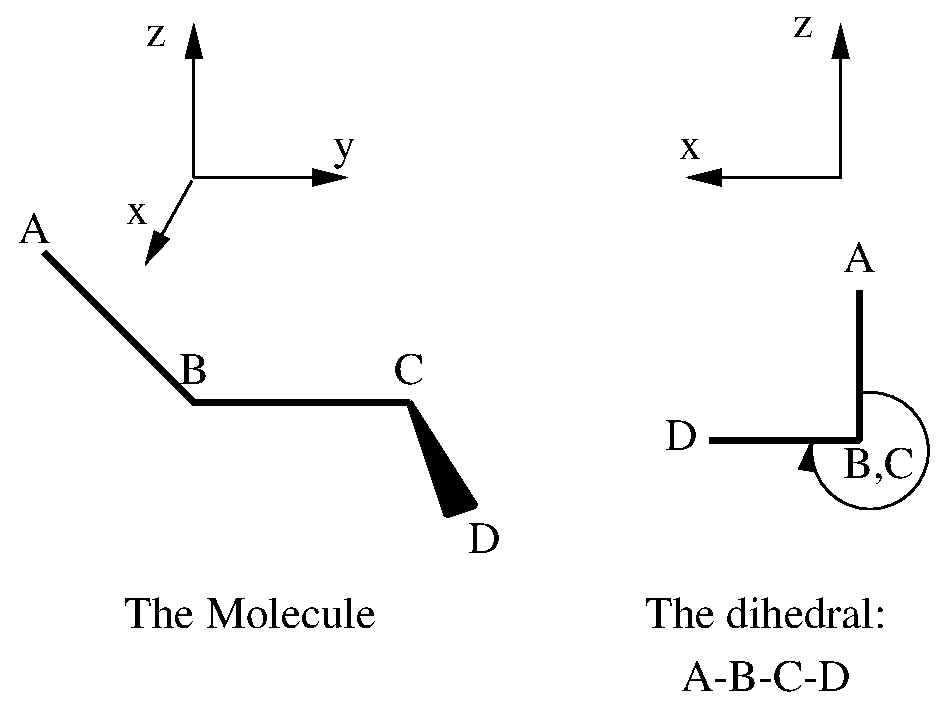
\epsfig{file=dihedral.eps,width=5.0in}
\end{center}
%

With that definition under our belt, here's the Geometry specification for a 
square pyramidal (CH$_3$)BiI$_4$ fragment, where the CH$_3$ group is
along the Z axis and the Bi and four I's lie in the XY plane:

\shrinkspacing
\begin{verbatim}
Geometry Z Matrix
9
1 Bi
2 C 1 2.1
3 I 1 2.7  2  90.0
4 I 1 2.7  2  90.0  3  90.0
5 I 1 2.7  2  90.0  3 180.0
6 I 1 2.7  2  90.0  3 270.0
7 H 2 1.1  1 109.5  3   0.0
8 H 2 1.1  1 109.5  3 120.0
9 H 2 1.1  1 109.5  3 240.0
\end{verbatim}
\resumespacing

Let's look at the first few entries in more detail.
\begin{enumerate}
\item The first atom is a Bi and it's placed at the origin.
Cartesian:  (0 0 0).  

\item Atom two is a C.  It's placed on the Z axis, 2.1 \AA\ away from
atom 1. Cartesian: (0 0 2.1).

\item Atom three is an I.  It's placed 2.7 \AA\ away from atom 1 and
the angle between atoms 3--1--2 in the XZ plane is 90.0 degrees.  
Cartesian: (2.7 0 0).

\item Atom four is an I.  It's placed 2.7 \AA\ away from atom 1, the
angle 4--1--2 is 90 degrees.  This angle puts us in the XY plane.  At
this point we know that atom 4 lies on a circle in the XY plane with
radius 2.7 \AA. The
dihedral 4--1--2--3 (90 degrees) tells us where on the circle we are. 
This dihedral is particularly easy to see:  if we look down the bond
2--1 (which is looking down the Z axis), the angle between the bond
3--1 and the bond 4--1 is 90 degrees.  So atom 4 lies on the Y axis.
Taking the right-handedness of dihedrals into account, we know that
atom 4 lies on the negative Y axis.  Cartesian (0 -2.7 0).

\item Atom five is an I.  It's 2.7 \AA\ away from atom 1, making an
angle of 90 degrees with 2 and a dihedral of 180 with 3.  This puts us
on the negative X axis.  Cartesian (-2.7 0 0).

\end{enumerate}

If you find the handedness of dihedrals confusing, just play around
with a couple of molecules defined using Z matrices, you'll get the
hang of it fairly quickly.



\begin{thebibliography}{20}


\bibitem{eht1} (a) R. Hoffmann, W. N. Lipscomb, J. Chem. Phys. {\bf 36}, 2179 (1962) {\it ibid} {\bf 36}, 3489 (1962) \\ (b) R. Hoffmann, W. N. Lipscomb, J. Chem. Phys. {\bf 37}, 2872 (1963) \\ (c) R. Hoffmann, J. Chem. Phys. {\bf 39}, 1397 (1963) \\ (d) R. Hoffmann, J. Chem. Phys. {\bf 40}, 2474 (1964) {\it ibid} {\bf 40}, 2745 (1964).

\bibitem{eht2} T. A. Albright, J. K. Burdett and M. -H. Whangbo, {\it Orbital Interactions in Chemistry} (Wiley-Interscience, 1985).

\bibitem{cohp1} R. Dronskowski, J. Am. Chem. Soc. {\bf 114}, 7230 (1992).

\bibitem{cohp2} R. Dronskowski and P. E. Bl\"{o}chl, J. Phys. Chem. {\bf 97}, 8617 (1993).

\bibitem{cohp3} W. V. Glassey, G. A. Papoian and R. Hoffmann, {\it accepted for publication in J. Chem. Phys.}

\bibitem{wolfsberg} M. Wolfsberg and L. Helmholtz, J. Chem. Phys. {\bf 20}, 837 (1952).

\bibitem{com1} M. -H. Whangbo and R. Hoffmann, J. Chem. Phys. {\bf 68}, 5498 (1978).

\bibitem{com2} J. H. Ammeter, H. -B. Burgi, J. C. Thibeault and R. Hoffmann, J. Am. Chem. Soc. {\bf 100}, 3686 (1978).

\bibitem{mulliken} R. S. Mulliken, J. Chem. Phys. {\bf 23}, 1841 (1955).

\bibitem{coop} T. Hughbanks and R. Hoffmann, J. Am. Chem. Soc. {\bf 105}, 3528 (1983).

\bibitem{thesis} G.A.Landrum, {\it Ph.D. dissertation}, Cornell University 1997 \\Greg's thesis is also available on the WWW via a link from the \prog home page: \\ {\it http://www.overlap.chem.cornell.edu:8080/yaehmop.html}

\bibitem{cod} E. Ruiz, S. Alvarez, R. Hoffmann and J. Bernstein, J. Am. Chem. Soc. {\bf 116}, 8207 (1994).

\end{thebibliography}

\end{document}


